%========= Methodology
\section{Methodology \& Discussion}

In this work, three types of thresholding was performed: Otsu, K-means and Gaussian. The HCC was calculated for all of them to check which method is the most accurate in terms of hydrides connectivity evaluation. Using GitHub to collaborate, we developed a Jupyter notebook from which the functions are called to show clarity in the script.

\noindent
The following sections were developed throughout the workflow:

\begin{enumerate}

    \item \textbf{Import packages.}
This sections is used to call all the packages needed to the correct running of the whole script.

    \item\textbf{ Import the images from GitHub.}
In this part of the code, the images to analyse are loaded.

    \item \textbf{Image processing.}
Because of the large area of the images being analysed, there are shadows that may lead us to incorrect results. To solve this, here it is included some code to break the image into vertical grayscale strips. The strips are also blurred and saved in their own directories.

    \item \textbf{Thresholding.}
In this part, the grayscale and blurred strips are transformed into binary images and three different thresholding methods are applied to see which one offers the best result:

\begin{itemize}
\item \textbf{Otsu thresholding}
\end{itemize}

\begin{itemize}
\item \textbf{K-means thresholding}
\end{itemize}

\begin{itemize}
\item \textbf{Thresholding - Gaussian}
\end{itemize}

Adaptive Gaussian thresholding was applied to binarize the image. Adaptive means that the levels for each thresholded pixel were chosen based on the surrounding pixels, in order to adapt the thresholding according to different levels of illumination or contrast on the image. Unfortunately, due to the complexity of the images and very different illumination conditions across the whole sample size, the result from adaptive Gaussian thresholding was extremely noisy and therefore, unsuitable for HCC analysis.

To mitigate this, erosion and dilation treatments were employed (provided by OpenCV), as well as area-based thresholding (removed an isolated island of pixels below a specified area threshold) (provided by skimage). Both methods were also combined for the sake of comparison. An example of what was obtained is shown in Figure X.

Based on qualitative analysis, the erosion and dilation treatment did very little on its own to improve the presence of noise on the binarized micrographs. The area-based thresholding had far greater success, with the connected hydride structures present in the original images becoming more clearly visible. Combining both treatments offered an improvement for images with more initial noise, but removed long hydrides for images with less initial noise. At this time, a method has not been developed that uses the best method for the appropriate image. Therefore, for any set of images, the method would have to be chosen qualitatively for each image. Hence, this method is too inconsistent to be considered useful for HCC analysis. 

    \item \textbf{Connectivity of microstructure.}
In this section, the connectivity between hydrides in the radial direction and the edges are detected to discover the contours within the slices. With this information, the HCC parameter of each strip is measured, and finally the average HCC value is obtained for each of the three thresholding methods.

    \item \textbf{Testing of functions.}
Testing the code in each function allows for a more robust execution of the code by integrating and automating the test procedure. Example micrographs created and modified with known will enable us to know what outputs to expect for each function's input. Comparing the similarity of images gives us a pass or fail criteria.By anticipating how the end-user might use the code and its environment, testing decreases the likelihood of unexpected errors. \par

Description of test methods:

\begin{itemize}


\item Processing: 
 
            \begin{figure}[h] 
            \centering
            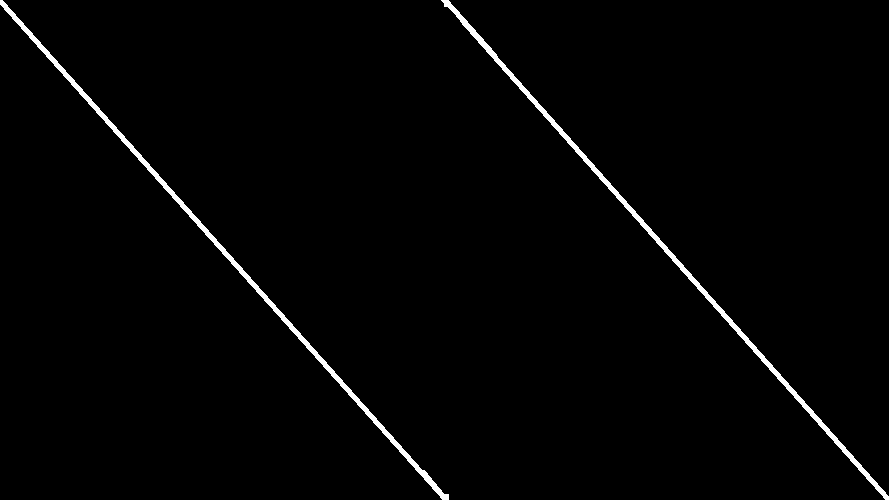
\includegraphics[width=2in]{Figures/testing/45Degrees.png}
            \caption{Test image with of 889 png by 500 png}
            \label{fig:processing_vertical_strips}
            \end{figure}   


    A test was made to check vertical strips produced in the program. The vertical strips function is one of the most important functions which enables the rest of the functions to work.
    Figure \ref{fig:processing_vertical_strips} was used with dimensions of 889 x 500 png. Processing.vertical\_strips() sections the image into equal sections by dividing the image width by an integer starting from 15. The function should only return the number 7. If it doesn't there is a problem with the code. 
    \item Connectivity:
    
    Connectivity.otsu() transforms grey-scale image like Figure \ref{fig:gradient_in} to a black and white image, Figure \ref{fig:Grad_Out}. By comparing the Numpy data array of the we can check the efficacy of the function.
    
    
    \noindent
        \begin{figure}
             \centering
             \begin{subfigure}[b]{0.3\textwidth}
                 \centering
                 
\includegraphics[width=\textwidth]{Figures/testing/Gradient.png}
                 \caption{Light to dark gradient used for testing thresholding calculation}
                 \label{fig:gradient_in}
             \end{subfigure}
             
             \begin{subfigure}[b]{0.3\textwidth}
                 \centering
                 
\includegraphics[width=\textwidth]{Figures/testing/Gradient_out.png}
                 \caption{Output image for test gradient}
                 \label{fig:Grad_Out}
             \end{subfigure}
            
            \caption{Input and Output Images for thresholding test}
            \label{fig:two gradients}
        \end{figure}
    
    \item Parameters:
        One of the main aims of the code was to find the Hydride Continuity factor of micrographs produced. Figure \ref{fig:test_image_hcc2} was the image chosen to check HCC value. By substituting the length of each hydride and total length of the strip in equation \ref{HCC_eqn} , equation \ref{test_hcc_eqn} is produced. This gives the expected return value of the HCC function when Figure \ref{fig:test_image_hcc2} is used.
        
        \begin{figure}[h] 
        \centering
        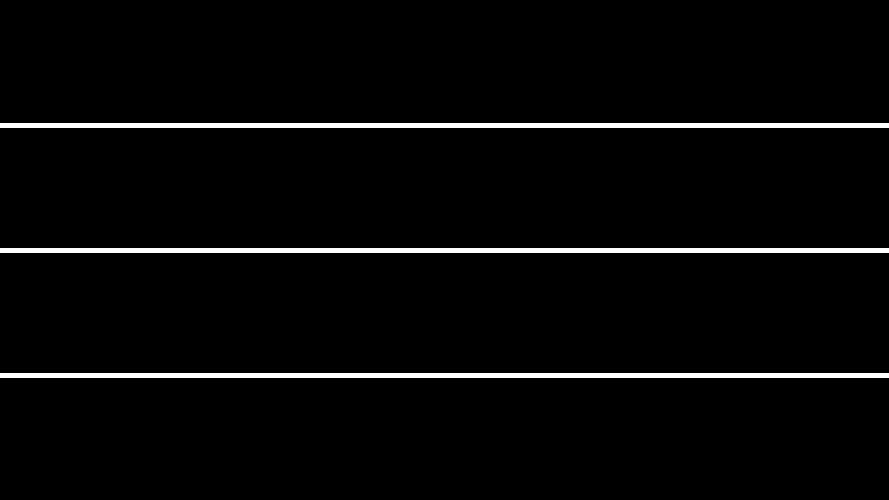
\includegraphics[width=2in]{Figures/testing/Full_Horizontal.png}
        \caption{Image to test HCC2 function}
        \label{fig:test_image_hcc2}
        \end{figure}
        
        \begin{equation} \label{test_hcc_eqn}
        \frac{3.68 + 3.68 + 3.68 }
                {133.86}
        = 0.0824742268
        \end{equation}
    
    \item For Gaussian thresholding two tests were created:
    
    \begin{enumerate}
        \item Tests whether after each treatment the input image and the output image had at least a 95\% similarity in terms of the image arrays. The test(s) was made to quickly determine whether a treatment (or its chosen parameters) had a large enough effect on the image to be considered useful.
        \item After the initial adaptive Gaussian thresholding, each pixel of the image was analyzed to determine whether it was white (value of 0) or black (value of 255). The test was made to confirm that the binarization had been successful and whether any possible subsequent treatment can rely on the fact the image is truly binary.
    
    \end{enumerate}
\end{itemize}


\end{enumerate}


